% Created 2019-01-14 Mon 23:38
% Intended LaTeX compiler: pdflatex
\documentclass[12pt, letterpaper]{paper}
\usepackage[utf8]{inputenc}
\usepackage[T1]{fontenc}
\usepackage{graphicx}
\usepackage{grffile}
\usepackage{longtable}
\usepackage{wrapfig}
\usepackage{rotating}
\usepackage[normalem]{ulem}
\usepackage{amsmath}
\usepackage{textcomp}
\usepackage{amssymb}
\usepackage{capt-of}
\usepackage{hyperref}
\usepackage{Schwieg}
\usepackage{natbib}
\usepackage{tikz}
\usepackage{bm}
\usepackage{minted}
\usepackage[margin=1in]{geometry}
\usepackage{fontspec}
\setmonofont{DejaVu Sans Mono}[Scale=MatchLowercase]
\author{Timothy Schwieg}
\date{\today}
\title{Structural Estimation Pset 2}
\hypersetup{
 pdfauthor={Timothy Schwieg},
 pdftitle={Structural Estimation Pset 2},
 pdfkeywords={},
 pdfsubject={},
 pdfcreator={Emacs 26.1 (Org mode 9.1.9)}, 
 pdflang={English}}
\begin{document}

\maketitle

\section{Question One}
\label{sec:org29dab38}
\subsection{a}
\label{sec:orged21076}
\begin{minted}[frame=lines,fontsize=\scriptsize,xleftmargin=\parindent,linenos,mathescape,breaklines=true,stripnl=true,firstnumber=last]{julia}
healthClaims = CSV.read( "clms.txt", header=[:A] )
describe( healthClaims )

println( "Standard Deviation: ", std(healthClaims[:A]))

histogram( healthClaims[:A], bins=1000, normalize = true)
savefig("histOne.png")
\end{minted}

\begin{center}
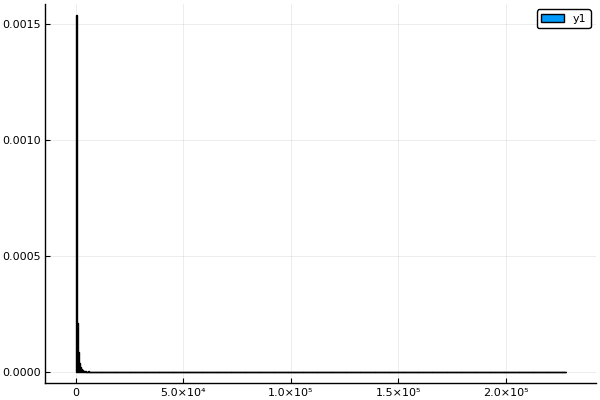
\includegraphics[width=.9\linewidth]{histOne.png}
\end{center}

\begin{minted}[frame=lines,fontsize=\scriptsize,xleftmargin=\parindent,linenos,mathescape,breaklines=true,stripnl=true,firstnumber=last]{julia}
truncatedHealthClaims = healthClaims[healthClaims[:A] .<= 800, 1]


histogram( truncatedHealthClaims, bins = 100, normalize = true)
savefig("histTwo.png")
\end{minted}

\begin{center}
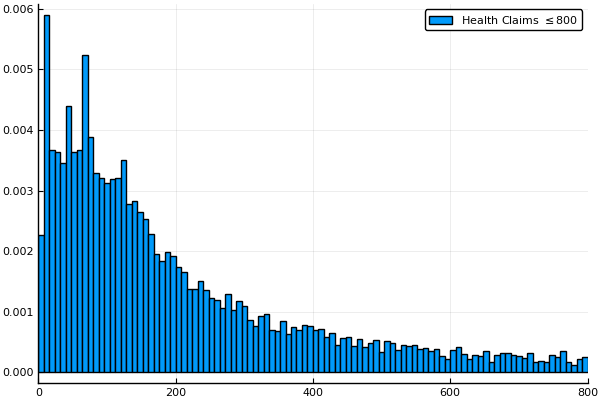
\includegraphics[width=.9\linewidth]{histTwo.png}
\end{center}



\subsection{b}
\label{sec:org1b60f50}
\begin{minted}[frame=lines,fontsize=\scriptsize,xleftmargin=\parindent,linenos,mathescape,breaklines=true,stripnl=true,firstnumber=last]{julia}
function GammaLogLikelihood( x::Vector{Float64}, α::Float64, β::Float64)
    #Yes I know I could get this using Distributions.jl which could
    #even do the MLE estimate But thats pretty much cheating, and
    #gamma is in the exponential family so using Newton's method will
    #cause no issues.

    #Pdf is: $\frac{ 1 }{\Gamma(\alpha) \beta^{\alpha}} x^{\alpha - 1} \exp\left( - \frac{x}{\beta} \right)$
    #Log-likelihood is: $- \alpha \log ( \beta) - \log( \Gamma (\alpha)) + (\alpha - 1) \log x - \frac{x}{\beta}$

    return -α*log( β) - lgamma(α) + (α - 1)*mean(log.(x)) - mean(x) / β
end

function GammaGradient( x::Vector{Float64}, α::Float64, β::Float64)
    delA = -log(β) - digamma(α) + mean(log.(x))
    #delB = mean(x) / β - α
    delB = mean(x) / β^2 - α / β
    return [delA,delB]
end

function GammaHessian( x::Vector{Float64}, α::Float64, β::Float64)
    delAA = -trigamma(α)
    delAB = -1 / β
    delBB =( α / (β*β)) - ((2* mean(x)) / (β*β*β))
    return [delAA delAB; delAB delBB]
end

function GammaPDF( α::Float64, β::Float64, x::Float64)
    return  (1 / (gamma(α)*β^α))*x^(α-1)*exp( -x/β)
end

function EstimateGammaParameters( data::Vector{Float64}, guess::Vector{Float64}, gradientFun, hessianFun)

    θ = guess
    tol = 1e-10
    maxLoops = 100

    grad = gradientFun( data, θ... )
    hess = hessianFun( data, θ... )

    loopCounter = 0
    while( loopCounter < maxLoops && norm(grad) >= tol)
        θ = θ - hess \ grad
        grad = gradientFun( data, θ... )
        hess = hessianFun( data, θ... )

        loopCounter += 1
        # println( norm(grad))
        # println( θ)
        # println( " ")
    end
    #println( loopCounter)
    return θ
end
healthCosts = convert(  Vector{Float64}, truncatedHealthClaims )#healthClaims[:A] )

β₀ =  var(healthCosts) / mean(healthCosts)
α₀ = mean(healthCosts) / β₀

(Gamma_̂α, Gamma_̂β) = EstimateGammaParameters( healthCosts, [α₀, β₀], GammaGradient, GammaHessian)

likelihood = GammaLogLikelihood(  healthCosts, Gamma_̂α, Gamma_̂β)

result = [["\$\\est{\\alpha}\$: ", "\$\\est{\\beta}\$: ", "Likelihood: " ] [ Gamma_̂α,  Gamma_̂β, likelihood]]


\end{minted}

\begin{center}
\begin{tabular}{lr}
\(\est{\alpha}\): & 1.1397564780585858\\
\(\est{\beta}\): & 174.8688733959653\\
Likelihood: & -6.28964508639924\\
\end{tabular}
\end{center}

\begin{minted}[frame=lines,fontsize=\scriptsize,xleftmargin=\parindent,linenos,mathescape,breaklines=true,stripnl=true,firstnumber=last]{julia}

histogram( truncatedHealthClaims, bins = 100, normalize = true)
pdfXVal = range( minimum(truncatedHealthClaims)+5, maximum(truncatedHealthClaims))
#pdfXVal = linspace( minimum(truncatedHealthClaims), maximum(truncatedHealthClaims))
pdfYVal = [GammaPDF( Gamma_̂α, Gamma_̂β, x ) for x in pdfXVal]


plot!( pdfXVal, pdfYVal, label="Gamma Estimate" )
savefig("histPDF_Gamma.png")
\end{minted}

\begin{center}
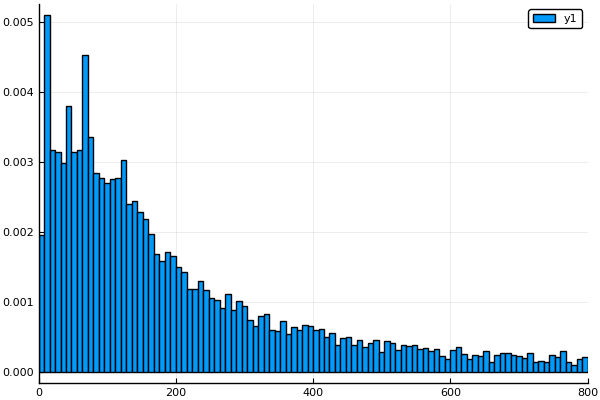
\includegraphics[width=.9\linewidth]{histPDF_Gamma.png}
\end{center}

\section{c}
\label{sec:orga90bcb5}
\begin{minted}[frame=lines,fontsize=\scriptsize,xleftmargin=\parindent,linenos,mathescape,breaklines=true,stripnl=true,firstnumber=last]{julia}

#I don't think this is the correct pdf?
function GGammaPDF( α::Float64, β::Float64, m::Float64, x::Float64)
    return ( (m / β^α) * x^(α-1) * exp( - (x / β)^m) ) / gamma( α / m)

    #return (m * x^(m*β - 1) * exp( - (x / α)^m))/ (α^(m*β) * gamma( β ) )
end


function GGammaLikelihood( x::Vector{Float64}, α::Real, β::Real, m::Real)
    return log(m) - α*log(β) + (α - 1)*mean(log.(x)) - mean( (x ./ β).^m  ) - lgamma( α / m )    
end

function EstimateGG( data::Vector{Float64}, guess::Vector{Float64})
    #To hard enforce that all of our parameters are positive, we
    #exponentiate them
    θ = log.(guess)
    fun(x::Vector) = -GGammaLikelihood( data, exp.(x)... )



    result = optimize(fun, θ, ConjugateGradient(), autodiff=:forward)
end

sln = EstimateGG( healthCosts, [Gamma_̂α, Gamma_̂β, 1.0])

GG_̂α = exp(sln.minimizer[1])
GG_̂β = exp(sln.minimizer[2])
GG_̂m = exp(sln.minimizer[3])
GG_LogLikelihood = -sln.minimum

println( "GG ̂α = ", GG_̂α)
println( "GG ̂β = ", GG_̂β )
println( "GG ̂m = ", GG_̂m )
println( "Likelihood Value: ", GG_LogLikelihood )

result = [["GG \$\\est{\\alpha}\$: ", "GG \$\\est{\\beta}\$: ", "GG \$\\est{m}\$: ","GG Likelihood: " ] [ GG_̂α,  GG_̂β,  GG_̂m, GG_LogLikelihood]]
\end{minted}

\begin{center}
\begin{tabular}{lr}
GG \(\est{\alpha}\): & 1.1755020098846642\\
GG \(\est{\beta}\): & 156.18446475134172\\
GG \(\est{m}\): & 0.9498167064643459\\
GG Likelihood: & -6.289560051458711\\
\end{tabular}
\end{center}

\begin{minted}[frame=lines,fontsize=\scriptsize,xleftmargin=\parindent,linenos,mathescape,breaklines=true,stripnl=true,firstnumber=last]{julia}
histogram( truncatedHealthClaims, bins = 100, normalize = true)
pdfXVal = range( minimum(truncatedHealthClaims), maximum(truncatedHealthClaims))
#pdfXVal = linspace( minimum(truncatedHealthClaims), maximum(truncatedHealthClaims))
pdfYVal = [GGammaPDF( GG_̂α, GG_̂β, GG_̂m, x ) for x in pdfXVal]

plot!( pdfXVal, pdfYVal, label="Generalized Gamma Estimate" )
savefig( "histPDF_GG.png" )
\end{minted}

\begin{center}
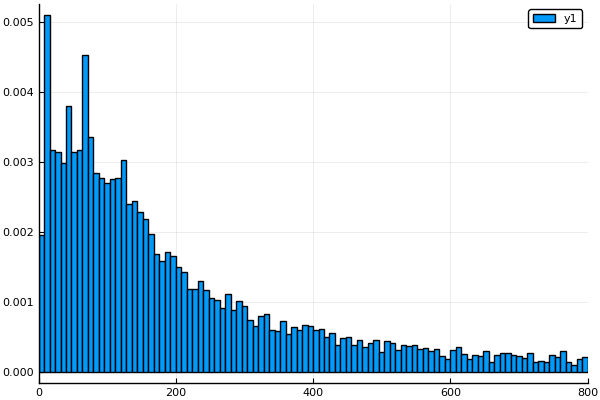
\includegraphics[width=.9\linewidth]{histPDF_GG.png}
\end{center}


\subsection{d}
\label{sec:orgaf92f24}
\begin{minted}[frame=lines,fontsize=\scriptsize,xleftmargin=\parindent,linenos,mathescape,breaklines=true,stripnl=true,firstnumber=last]{julia}
function GBetaTwoPDF( x::Float64, a::Real, b::Real, p::Real, q::Real)
    #We require all parameters to be positive, so abs(a) = a
    return a*x^(a*p -1) / (b^(a*p) *beta(p,q)*(1+(x/b)^a)^(p+q))
end

function GBetaTwoLikelihood( x::Vector{Float64}, a::Real, b::Real, p::Real, q::Real)
    return log( a) + (a*p -1)*mean(log.(x)) - (a*p)*log(b) - log(beta(p,q)) - (p+q)*mean( log.( 1 .+(x ./ b).^a ))
end

function EstimateGBetaTwo( data::Vector{Float64}, guess::Vector{Float64})
      #To hard enforce that all of our parameters are positive, we
      #exponentiate them
    θ = log.(guess)
    #θ = guess
    fun(x::Vector) = -GBetaTwoLikelihood( data, exp.(x)... )


    #This guy is being fickle, and Newton() would not converge
    #LBFGS converges, but to a higher value than Newton()
    result = optimize(fun, θ, NewtonTrustRegion(), autodiff=:forward, Optim.Options(iterations=2000) )
end

sln = EstimateGBetaTwo( healthCosts, [GG_̂α, GG_̂β, GG_̂m, 10000])

GB2_̂α = exp( sln.minimizer[1])
GB2_̂β = exp( sln.minimizer[2])
GB2_̂p = exp( sln.minimizer[3])
GB2_̂q = exp( sln.minimizer[4])
GB2_LogLikelihood = -sln.minimum

result = [["GB2 \$\\est{\\alpha}\$: ", "GB2 \$\\est{\\beta}\$: ", "GB2 \$\\est{p}\$: ","GB2 \$\\est{q}\$: ","GB2 Likelihood: " ] [GB2_̂α, GB2_̂β,  GB2_̂p,  GB2_̂q, -sln.minimum]]
\end{minted}

\begin{center}
\begin{tabular}{lr}
GB2 \(\est{\alpha}\): & 0.9498180950429491\\
GB2 \(\est{\beta}\): & 1.0983701276884081\,(9)\\
GB2 \(\est{p}\): & 1.2376067626960379\\
GB2 \(\est{q}\): & 3.187929333688613\,(6)\\
GB2 Likelihood: & -6.289560054356965\\
\end{tabular}
\end{center}

\begin{minted}[frame=lines,fontsize=\scriptsize,xleftmargin=\parindent,linenos,mathescape,breaklines=true,stripnl=true,firstnumber=last]{julia}
histogram( truncatedHealthClaims, bins = 100, normalize = true)
pdfXVal = range( minimum(truncatedHealthClaims), maximum(truncatedHealthClaims))
#pdfXVal = linspace( minimum(truncatedHealthClaims), maximum(truncatedHealthClaims))
pdfYVal = [GBetaTwoPDF( x, GB2_̂α, GB2_̂β, GB2_̂p, GB2_̂q ) for x in pdfXVal]

plot!( pdfXVal, pdfYVal, label="Generalized Beta 2 Estimate" )
savefig( "histPDF_GB2.png" )
\end{minted}

\begin{center}
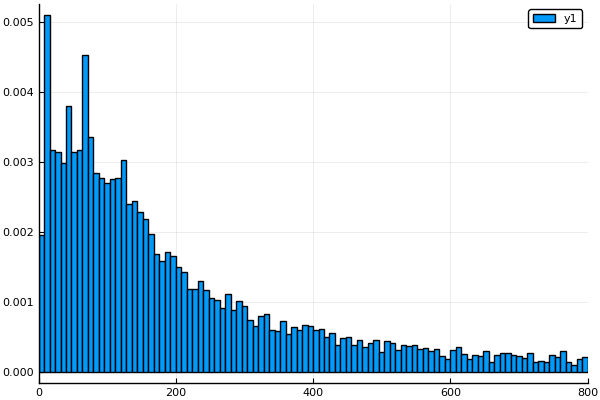
\includegraphics[width=.9\linewidth]{histPDF_GB2.png}
\end{center}

\subsection{e}
\label{sec:org13cb78f}
Since the likelihood function values at the optimum for parts (b) and
(c) are the constrained maximum likelihood estimators, the likelihood
ratio test is simply: 
\begin{equation*}
  2 \left( f( \est{\theta} - \altest{\theta}) \right) \sim \chi_{p}^{2}
\end{equation*}

Where \(p\) is the number of constraints in the estimation procedure. 
\begin{minted}[frame=lines,fontsize=\scriptsize,xleftmargin=\parindent,linenos,mathescape,breaklines=true,stripnl=true,firstnumber=last]{julia}

# Gamma Has Two restrictions
tStatGamma = 2*(GB2_LogLikelihood - likelihood)
# Generalized Gamma Has One Restriction
tStatGG = 2*(GB2_LogLikelihood - GG_LogLikelihood)

results = [["", "Gamma", "Generalized Gamma"] [ "\$\\chi^{2}\$", tStatGamma, tStatGG] ["p-value",  cdf(Chisq(2),tStatGamma), cdf( Chisq(1),tStatGG) ] ]
\end{minted}

\begin{center}
\begin{tabular}{lrr}
 & \(\chi^{2}\) & p-value\\
Gamma & 0.00017006408454989241 & 8.502842715330726\,(-5)\\
Generalized Gamma & -5.796508162347891\,(-9) & 0.0\\
\end{tabular}
\end{center}

\subsection{f}
\label{sec:orgb8fa7b1}
The Probability that someone has a health care claim of more than
$\backslash$$1000 is given by:

\begin{align*}
  \Pr( X > 1000) &= 1 - \Pr( X \leq 1000)\\
                 &= \int_0^{1000}f_Xdx
\end{align*}

However, since the integral of a Generalized Beta 2 Distribution is
quite nasty, we will compute it numerically.

\begin{minted}[frame=lines,fontsize=\scriptsize,xleftmargin=\parindent,linenos,mathescape,breaklines=true,stripnl=true,firstnumber=last]{julia}
f(x) = GBetaTwoPDF( x, GB2_̂α, GB2_̂β, GB2_̂p, GB2_̂q )
area = quadgk( f, 0, 1000 )[1]
output = ["Probability of Having > 1000: " (1-area)]
\end{minted}

\begin{center}
\begin{tabular}{lr}
Probability of Having > 1000: & 0.00507829692428996\\
\end{tabular}
\end{center}



\section{Question 2}
\label{sec:org3931c06}

\subsection{a}
\label{sec:org3f70910}

Equations (3) and (5) tell us that


\begin{align*}
  w_t - (1-\alpha) exp( z_t ) (k_t)^{\alpha-1} &= 0\\
  z_t = \rho z_{t-1} + (1-\rho)\mu &+ \epsilon_t
\end{align*}


Note that: $z_0 = \mu$ Therefore:
\begin{align*}
  z_1 &= \mu + \epsilon_1\\
  z_2 &= \mu + \rho\epsilon_1 + \epsilon_2\\
  z_t &= \mu + \sum_{i=0}^{t-1} \rho^i \epsilon_{t-i}
\end{align*}

Combining these two together:

\begin{equation*}
  w_t - (1-\alpha) exp \left( \mu + \sum_{i=0}^{t-1} \rho^i \epsilon_{t-i} \right) k_t^{\alpha} = 0
\end{equation*}

Taking logs and isolating the random component:
\begin{equation*}
  \log w_t - \log(1-\alpha) - \mu - \alpha \log k_t =  \sum_{i=0}^{t-1} \rho^i \epsilon_{t-i}
\end{equation*}

Note that the sum of iid distributed normal random variables is
distributed normal, where the variance is given by the sum of the
variances.

Thus
\begin{equation*}
  \sum_{i=0}^{t-1} \rho^i \epsilon_{t-i} \sim \normal( 0, \sigma^2 \sum_{i=0}^{t-1} \rho^{2i}) =
  \normal\left( 0, \sigma^2 \frac{1 - \rho^{2i}}{1-\rho}\right)
\end{equation*}

We may now estimate this model using Maximum Likelihood Estimation

\begin{minted}[frame=lines,fontsize=\scriptsize,xleftmargin=\parindent,linenos,mathescape,breaklines=true,stripnl=true,firstnumber=last]{julia}
#$\log w_t - \log(1-\alpha) - \mu - \alpha \log k_t =  \sum_{i=0}^{t-1} \rho^i \epsilon_{t-i}$
# Variance of error: $\sigma^2 \frac{1 - \rho^{2i}}{1-\rho}$

#Clean it up when it exists, comes in the order: (c, k, w, r)
macroData = CSV.read( "MacroSeries.txt", header=[:C,:K,:W,:R])

w = convert( Vector{Float64}, macroData[:W] )
k = convert( Vector{Float64}, macroData[:K] )

function LogLikelihood( N, w::Vector{Float64}, k::Vector{Float64}, α::Real, ρ::Real, μ::Real, σ²::Real  )
    #The pdf of a normal: $\frac{1}{\sqrt{2 \pi \sigma^2}} \exp( - \frac{ (x-\mu)^2}{2 \sigma^2})$
    #Log Likelihood: $- \frac{1}{2} \log \sigma^2 - \frac{ (x-\mu)^2}{ 2 \sigma^2}$

    logLik = 0.0
    #Note the way that the model is structured is: F(...) = 0, so we
    #are maximizing the likelihood of getting a 0 returned for all the
    #moments

    #Note we do not have the -.5*log(2*pi)
    #Because that does not matter at all for MLE estimation.
    for i in 1:N
        mean = log(w[i]) - log( 1 - α) - μ - α*log( k[i])
        var = σ² * ( 1 - ρ^(2*i)) / ( 1 - ρ)
        logLik += -.5*log( σ² ) - (  mean*mean / (2*σ²))
    end
    return logLik
end

N = length(w)

α₀ = .5
β = .99
μ₀ = 1.0
σ₀ = 1.0
ρ₀ = 0.0

#We parameterize each of the variables so that they meet their constraints.
# tanh is used to ensure that $\rho \in (-1,1)$
θ = zeros(4)
θ[1] = log( α₀ / ( 1 - α₀) )
θ[2] = atanh( ρ₀)
θ[3] = log( μ₀ )
θ[4] = log( σ₀)


fun(x::Vector) = -LogLikelihood( N, w, k, exp(x[1]) / (1 + exp(x[1])), tanh(x[2]), exp(x[3]), exp(x[4])  )

result = optimize(fun, θ, LBFGS(), autodiff=:forward)

model_̂θ = result.minimizer

model_̂α = exp(model_̂θ[1]) / (1 + exp(model_̂θ[1]))
model_̂ρ = tanh(model_̂θ[2])
model_̂μ = exp(model_̂θ[3])
model_̂σ = exp(model_̂θ[4])

output = [["\$\\est{\\alpha}\$:", "\$\\est{\\rho}\$:", "\$\\est{\\mu}\$:", "\$\\est{\\sigma^{2}}\$:"]  [model_̂α, model_̂ρ, model_̂μ, model_̂σ]]
\end{minted}

\begin{center}
\begin{tabular}{lr}
\(\est{\alpha}\): & 0.9999999999985967\\
\(\est{\rho}\): & 0.0\\
\(\est{\mu}\): & 27.626774841787046\\
\(\est{\sigma^{2}}\): & 0.01003725876812115\\
\end{tabular}
\end{center}

\section{b}
\label{sec:org8c33180}

Equations (4) and (5) read:
\begin{align*}
  r_t - \alpha \exp( z_t ) k_t^{\alpha -1 } &= 0\\
  z_t = \rho z_{t-1} + (1-\rho)\mu &+ \epsilon_t\\
  \epsilon_t \sim \normal( 0, \sigma^2)
\end{align*}

From part (a) we know that (5) can be recursively solved to yield:
\begin{equation*}
  z_t \sim \normal\left( \mu, \sigma^2 \frac{1 - \rho^{2i}}{1-\rho}\right)
\end{equation*}

Solving for $r_t$ then taking logs in equation (4)
\begin{align*}
  \log r_t &= \log \alpha + z_t + (\alpha - 1 ) \log k_t\\
\end{align*}

This can be written as:
\begin{equation*}
  F( r_t, k_t, \alpha, \mu, \sigma, \rho ) = 0
\end{equation*}

where the variance of the random variable described by $F$ is known,
and the same as the variance of $z_t$. Thus this system can be
estimated by MLE.

\begin{minted}[frame=lines,fontsize=\scriptsize,xleftmargin=\parindent,linenos,mathescape,breaklines=true,stripnl=true,firstnumber=last]{julia}
r = convert( Vector{Float64}, macroData[:R] )
k = convert( Vector{Float64}, macroData[:K] )

#$\log r_t - \log \alpha - z_t - (\alpha - 1 ) \log k_t = 0$

function LogLikelihood( N, w::Vector{Float64}, k::Vector{Float64}, α::Real, ρ::Real, μ::Real, σ²::Real  )
    #The pdf of a normal: $\frac{1}{\sqrt{2 \pi \sigma^2}} \exp( - \frac{ (x-\mu)^2}{2 \sigma^2})$
    #Log Likelihood: $- \frac{1}{2} \log \sigma^2 - \frac{ (x-\mu)^2}{ 2 \sigma^2}$

    logLik = 0.0
    #Note the way that the model is structured is: F(...) = 0, so we
    #are maximizing the likelihood of getting a 0 returned for all the
    #moments

    for i in 1:N
        mean = log(r[i]) - log( α) - μ - (α - 1)*log( k[i])
        var = σ² * ( 1 - ρ^(2*i)) / ( 1 - ρ)
        logLik += -.5*log( σ² ) - (  mean*mean / (2*σ²))
    end
    return logLik
end

N = length(w)

α₀ = .5
β = .99
μ₀ = 1.0
σ₀ = 1.0
ρ₀ = .99

#We parameterize each of the variables so that they meet their constraints.
# tanh is used to ensure that $\rho \in (-1,1)$
θ = zeros(4)
θ[1] = log( α₀ / ( 1 - α₀) )
θ[2] = atanh( ρ₀)
θ[3] = log( μ₀ )
θ[4] = log( σ₀)


fun(x::Vector) = -LogLikelihood( N, w, k, exp(x[1]) / (1 + exp(x[1])), tanh(x[2]), exp(x[3]), exp(x[4])  )

result = optimize(fun, θ, Newton(), autodiff=:forward)

model_̂θ = result.minimizer

model_̂α = exp(model_̂θ[1]) / (1 + exp(model_̂θ[1]))
model_̂ρ = tanh(model_̂θ[2])
model_̂μ = exp(model_̂θ[3])
model_̂σ = exp(model_̂θ[4])

output = [["\$\\est{\\alpha}\$:", "\$\\est{\\rho}\$:", "\$\\est{\\mu}\$:", "\$\\est{\\sigma^{2}}\$:"]  [model_̂α, model_̂ρ, model_̂μ, model_̂σ]]
\end{minted}

\begin{center}
\begin{tabular}{lr}
\(\est{\alpha}\): & 0.8887650406380285\\
\(\est{\rho}\): & 0.99\\
\(\est{\mu}\): & 1.8877579805483233\\
\(\est{\sigma^{2}}\): & 0.009515136163054447\\
\end{tabular}
\end{center}

\subsection{c}
\label{sec:org4cb7b57}
From the derivation of the distribution of $\log r_t$ in part (b):

\begin{align*}
    \Pr( r_t > 1) &= \Pr( \log r_t > 0)\\
                  &= \Pr( \log \alpha + z_t + (\alpha - 1)\log k_t > 0)\\
                  &= \Pr( \log \alpha + \rho z_{t-1} + (1 - \rho)\mu + \epsilon_t + (\alpha-1) \log k_t > 0)\\
    &= \Pr( \log(\alpha) + \rho z_{t-1} + (1-\rho)\mu + \frac{Z}{\sigma} + (\alpha-1) \log k_t
      > 0)\\
                  &= \Pr( Z > - \sigma ( \log(\alpha) + \rho z_{t-1} + (1-\rho)\mu + (\alpha-1)\log k_t))\\
    &= 1 - \Pr( Z \leq - \sigma ( \log(\alpha) + \rho z_{t-1} + (1-\rho)\mu + (\alpha-1)\log
      k_t))\\
                  &= \inv{ \Phi}( - \sigma ( \log(\alpha) + \rho z_{t-1} + (1-\rho)\mu + (\alpha-1)\log k_t ))\\
    &\approx \inv{\Phi}( -\est{\sigma} ( \log \est{\alpha} + \est{\rho}10 + (1-\est{\rho})
      \est{\mu} + (\est{\alpha} - 1) \log( 7,500,000) ))\\
  \end{align*}

\begin{minted}[frame=lines,fontsize=\scriptsize,xleftmargin=\parindent,linenos,mathescape,breaklines=true,stripnl=true,firstnumber=last]{julia}
  prob = cdf( Normal(), -sqrt(model_̂σ)*( log(model_̂α) + model_̂ρ*10 + (1-model_̂ρ)*model_̂μ + (model_̂α-1)*log( 7500000)))
result = ["Prob" prob]
\end{minted}

\begin{center}
\begin{tabular}{lr}
Prob & 0.21644022445230773\\
\end{tabular}
\end{center}
\end{document}